\chapter{Automatisierte dynamische Softwaretests}
\label{sec:test}
Zum Prüfen der Richtigkeit seiner Arbeit macht jeder Programmierer mindestens manuelle Tests. Bei einer Webanwendung hieße dies konkret, den Webserver zu starten und mittels eines Browsers durch die Anwendung zu navigieren, Daten anzulegen und Ausgaben der Anwendung zu kontrollieren. Mit zunehmender Größe einer Anwendung wird es immer aufwändiger, die Software zu testen, da nach jedem Hinzufügen von Funktionalität eigentlich alle Aspekte wieder getestet werden müssten, um Regressionsfehler auszuschließen.

Stattdessen werden \textbf{automatisierte Softwaretests} genutzt, um auf Knopfdruck alle bisher programmierten Tests auszuführen und so ein Bild über den Zustand der Anwendung zu erhalten. So ist automatisiertes Testen dem manuellem Testen, das auch \textbf{Ad-Hoc-Testen} genannt wird, in kürzester Zeit zeitlich überlegen \citep{rappin_rails_2011}.

Dynamische Testverfahren, also Tests die Programmcode ausführen und Ergebnisse beobachten, haben gemeinsam, dass sie stichpunktartig testen, damit die Korrektheit des Programmes nicht beweisen können und stattdessen den Programmcodes mit konkreten Eingabewerten ausführen \citep[S. 49]{liggesmeyer_modultest_1990}. Diese Stichproben werden als \textbf{Testdaten\index{Test!Testdaten}} bezeichnet, die optimalerweise repräsentativ, fehlersensitiv, redundanzarm und ökonomisch sind \citep[S. 51]{liggesmeyer_modultest_1990}.

Neben den \textbf{dynamischen Tests}, gibt es statische Analyseverfahren, wie formale Verifikation, symbolische Testverfahren oder statische Analysen. Einige statische Analysen werden später im Abschnitt \ref{sec:metrics} vorgestellt. Andere statische Testverfahren sind nicht Gegenstand dieser Diplomarbeit.

\section{Motivation zum Testen}
Weshalb sollte überhaupt Zeit dafür aufgewendet werden, um Software zu Testen?\\
Aus funktionaler Sicht dienen Tests in erster Linie dazu, das Vorhandensein bzw. Nichtvorhandensein von Software-Fehlern zu belegen \citep{goodliffe_code_2006}.\\
Aber das Testen hat auch weitere Auswirkungen auf die Software-Entwicklung: Testen führe zu einer Minimierung der Debugphase und mache die Software\hyp{}Entwicklung für Programmierer attraktiver und für Projektleiter leichter zu planen \citep{orsini_rails_2007} und insgesamt preiswerter \citep[S.13]{liggesmeyer_modultest_1990}.\\
Außerdem gilt getester Code im Allgemeinen als robuster, korrekter und leichter zu warten \citep{rappin_rails_2011}. Im Umkehrschluss bedeutet dies, dass ungetestete Software mit sehr hoher Wahrscheinlichkeit \glossar{fehler} beinhaltet \citep{goodliffe_code_2006}.

%TODO Kent Beck?

\section{Arten von Tests}
Tests können nach verschiedenen Gesichtspunkten eingeteilt werden. In vielen konkreten Fällen reich eine eindimensionale Einordnung nicht aus und Test \index{Test}können ebenso Teil mehrerer Kategorien sein. Einige der gängisten Einordnungen werden hier vorgestellt.
\begin{figure}[hp]
 \centering
 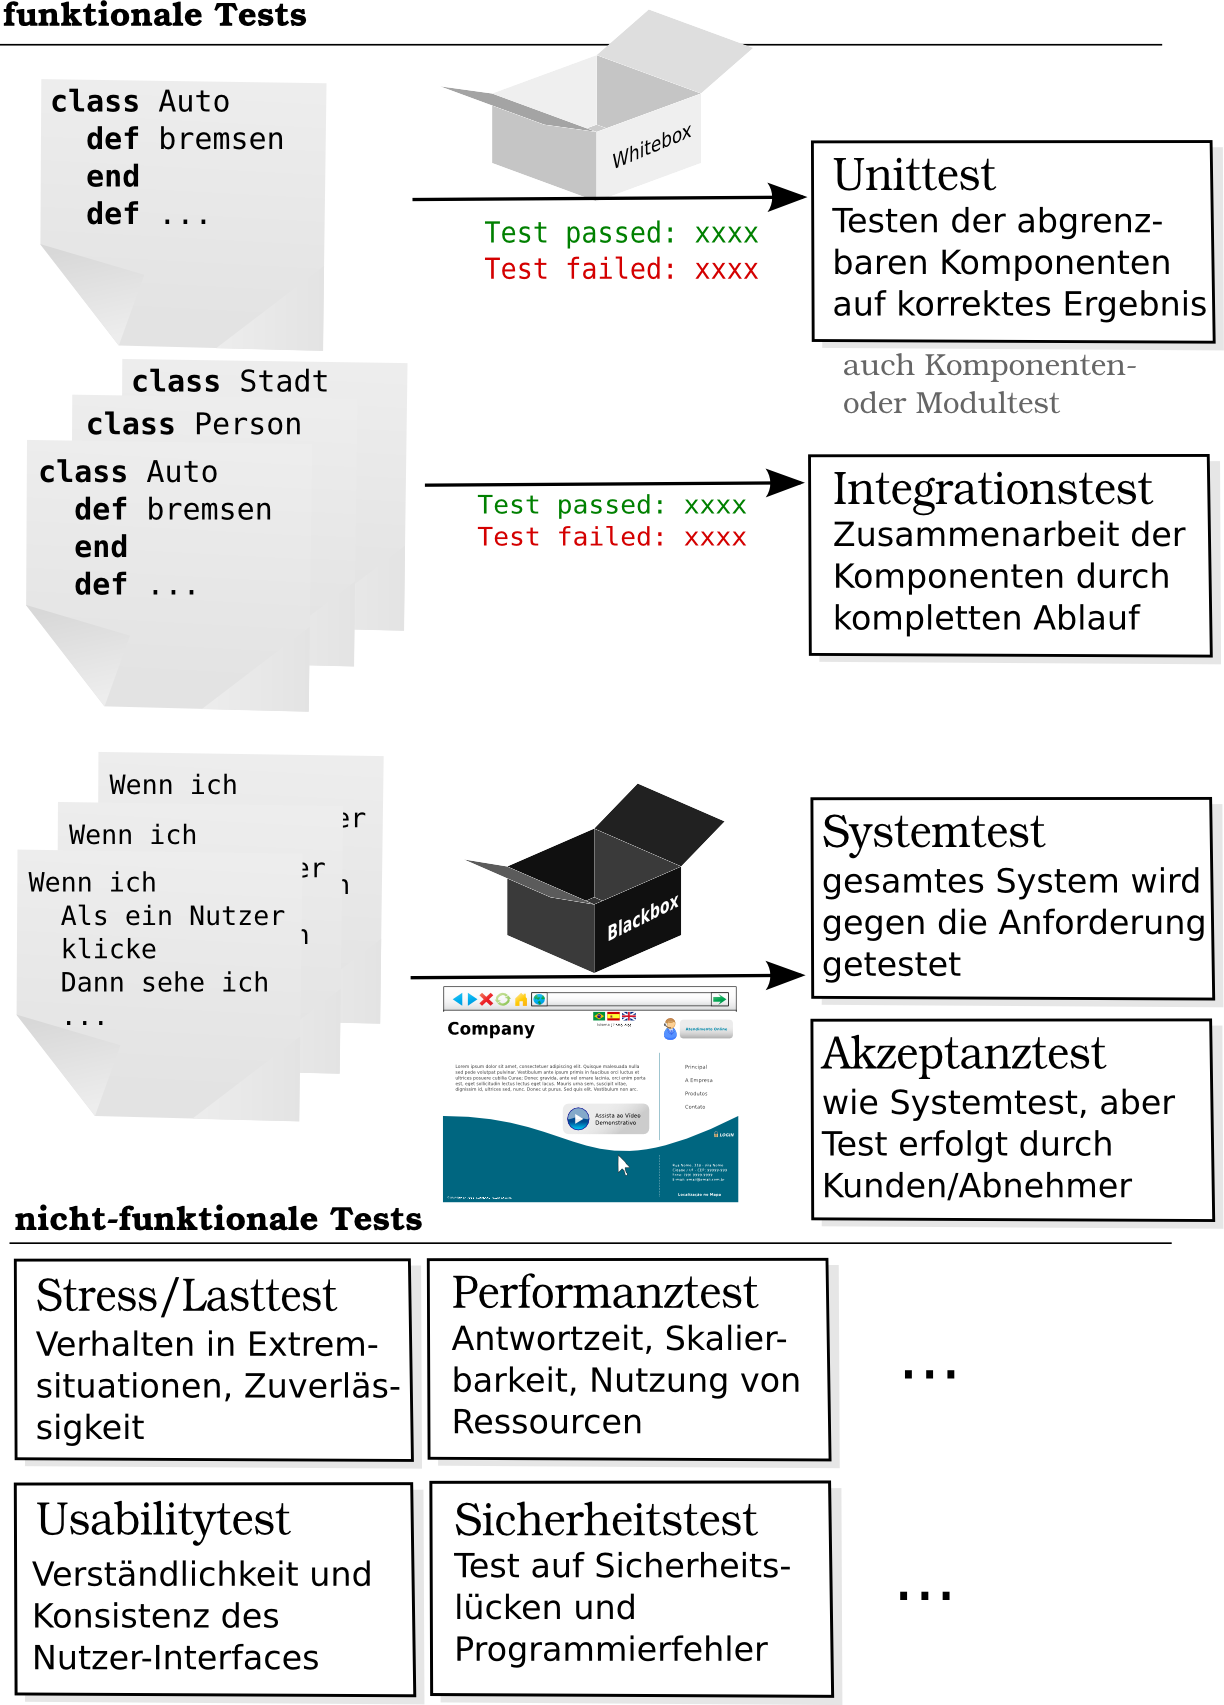
\includegraphics[width=\textwidth]{./diagrams/testarten.png}
 % testarten.pdf: 0x0 pixel, 300dpi, 0.00x0.00 cm, bb=
 \caption{Einteilung der Tests}
 \label{fig:testArten}
\end{figure}

\paragraph{Einteilung nach Sichtbarkeit des Quellcodes} Tests werden in \textbf{Whitebox}- und \textbf{Blackbox}-Tests eingeteilt.
Whitebox-Tests finden mit Wissen über den zugrundeliegenden Code statt. Ziel eines Whitebox-basierten Testverfahrens ist es, soviele Codeabschnitt wie möglich zu testen.\\
Blackbox-tests dagegen ignorieren den inneren Aufbau der Klassen und testen entweder nur Schnittstellen oder das Gesamtsystem und beobachten Rückmeldungen des Systems auf bestimmte Aktionen. Das Ziel eines Blackbox-basierten Tests ist es, die Korrektheit der Software gegenüber den Spezifikationen zu bestimmen.\\
Ein Spezialfall ist der sogenannte \textbf{Greybox}-Test, der insbesondere bei der Testgetriebene\index{TDD}n Entwicklung auftritt. Da hier der Test \index{Test}zuerst entwickelt wird, ist noch kein Wissen über den Zielquellcode vorhanden, der Entwickler aber natürlich Einblick in den Quellcode hat.

\paragraph{Einteilung nach Testziel} (nach \citep[S. 238ff]{hunt_pragmatic_1999})
\begin{description}
 \item[Unittest\index{Test!Unittest}s] Hierbei werden die Einheiten des Programmes auf ihr Verhalten getestet. Dies stellt die Basis für die meist darauffolgenden Integrationstests dar. Dieser wird ausführlich im nächsten Abschnitt behandelt
 \item[Integrationstests]  das Zusammenspiel zwischen Klassen wird getestet, welche ein gemeinsames Subsystem darstellen (Modul). Hier kann eine Bottom-Up oder Top-Down\hyp{}Integrationsstrategie verfolgt werden, d.h. ob man mit denjenigen Modulen beginnt, die keine Abhängigkeiten haben und im Ableitungsbaum immer weiter nach oben integriert (Bottom-Up) oder mit dem zentralen Modul anfängt und nach und nach alle abhängigen oder abgeleiteten Module testet (Top-Down) \citep{liggesmeyer_modultest_1990}.
 \item[Validierung und Verifikation] Testet den Fortschritt der Anwendung in Bezug auf die funktionalen Anforderungen. Dies ist meist ein Blackboxtest und testet das System als ganzes (=Systemtest). Ein Spezialfall ist der \textbf{Akzeptanztest\index{Akzeptanztest}}. Hierbei nimmt der Kunde eine Anforderung/Feature ab. Auch diesem Testtyp ist ein Unterabschnitt gewidmet.
 \item[Ressourcennutzung, Performanz, Verhalten im Fehlerfall] Die vorherigen genannten Testarten finden i.d.R. unter idealen Bedingungen statt. Diese Testkategorie nun versucht das Applikationsverhalten unter realen Bedingungen zu simulieren. Beim Verhalten im Fehlerfall soll getestet werden, dass der Nutzer nicht durch kryptische Fehlermeldungen verwirrt wird oder z.B. sein Fortschritt gespeichert wurde. Last und Performanztests stellen sicher, dass die Anwendung eine große Zahl von Nutzern oder eine große Menge an Daten verarbeiten kann.
 \item[Usability Testing] Diese Testmethode kann gegenüber den bisher genannten nicht automatisiert werden und benötigt immer einen zukünftigen Endanwender. Ziel ist es, die Benutzbarkeit und Handhabung zu testen. Dies wird durch Beobachtung von Kandidaten, meist in einer präperierten Umgebung (Usability Labor) geprüft.
\end{description}

\paragraph{Einteilung nach Testvollständigkeit} Auf welche Art die sogennante Testvollständigkeit beurteilt wird und notwendige Testfälle generiert werden, ist ebenfalls eine Möglichkeit, Tests \index{Test}einzuordnen \citep{liggesmeyer_modultest_1990}:
\begin{description}
 \item[Kontrollflussorientierter Test] betrachtet den Quelltext und leitet daraus notwendige Unittest\index{Test!Unittest}s ab
 \item[Datenflussorientierter Test] Beobachtet die Variablendefinitionen, Zugriffe und Entscheidungen anhand der Variablen
 \item[Funktionaler Test] leitet aus den funktionalen Spezifikationen Testfälle her und prüft, ob das Programm die Spezifikationen erfüllt
 \item[Diversifizierender Test] Testet verschiedene Versionen eines Programmes gegeneinander. Dies beinhaltet z.B. Mutationentest, der später im Abschnitt \ref{sec:mutation} \textit{\nameref{sec:mutation}} als Möglichkeit zur Beurteilung von Tests erläutert wird.
\end{description}
\section{Unittest}
\label{sec:testUnit}
Da die Testgetriebene\index{TDD} Entwicklung in ihrer Reinform auf dem Unittest\index{Test!Unittest} basiert, soll diese Testgattung im Vorfeld etwas näher beleuchtet werden.

Ziel des Unittest\index{Test!Unittest}s ist es, frühzeitig \glossar{fehler} im Code zu finden. Der Unit- oder Modultest beschreibt das Testen der Einheiten eines Programms, die im Sinne der Testung nicht weiter zerlegt werden können. Dies können die Funktionen oder bei einer objektorientierten Sprache, die Klassen sein. Die Objekte unter Beobachtung (Objects under Test) werden beim Unittest in strenger Isolation zu den restlichen Units ausgeführt. Abhängigkeiten der Module untereinander und von unterlagerten Diensten werden durch \glossarpl{Test-Double}\index{Test-Double} simuliert. Dies ist notwendig um sicherzustellen, dass gefundende Fehler von dem betreffendem Modul verursacht wurden und nicht durch äußere Einflüsse. Diese Isolierung macht das Testen einfacher \citep{goodliffe_code_2006,liggesmeyer_modultest_1990}.



Unittest\index{Test!Unittest}s werden fast immer durch sog. \glossar{testrunner} automatisiert ausgeführt. Außerdem werden meist Test-Frameworks verwendet, welche häufige Aufgaben beim Testen unterstützen, z.B. Auswertung der Testergebnisse, Integration der Tests mit dem Programmcode, Anlage und Löschen von Testdaten\index{Test!Testdaten}.  Eine der meist-verbreitetsten sind die Frameworks auf Basis von xUnit, die in nahezu allen (objektorientierten) Sprachen Vertreter haben, so z.B. Test/Unit\index{Test/Unit-Framwork}/MiniTest in Ruby\index{Ruby}, JUnit in Java oder NUnit in C\#.

Ein solcher Test \index{Test}besteht in der Regel aus 4 Teilen \citep{rappin_rails_2011} \citep[Karte 46]{langr_agile_2011}:
\begin{enumerate}
 \item Initialisierung der \glossar{Test-Umgebung} und der Objekte. Man arrangiert einen Kontext, der notwendig ist, um den zu Code ausführen zu können.
 \item Ausführung der zu testenden Aktion, die den Systemzustand ändert
 \item Prüfen der spezifizierten Erwartungen durch Zusicherungen (Assertions): prüfen, ob das System under Test/Object under Test \index{Test}sich wie erwartet verhalten hat.
 \item Aufräumen nicht mehr benötigter Objekte, File-Pointer, Sockets, Leeren der Datenbank\index{Datenbank} u.ä
\end{enumerate}
Als Faustregel für übersichtliche und nachvollziehbare Tests, gilt das Arrange-Act-Assert Konzept: Dabei werden die oben genannten Phasen als Arrange (1. u. 4.), Act (2.), Assert (3.) oder auch Given-When-Then (Angenommen, Wenn, Dann) bezeichnet \citep[Karte 46]{langr_agile_2011}. Nicht immer sind alle drei bzw. vier Teile notwendig.

\paragraph{Komponententest}
Ziel des Komponententests ist es, verschiedene Units in Kombination als eine vollständige Komponente zu testen \citep{goodliffe_code_2006}.

 \section{Test Doubles -- Mocks und Stubs}
  \label{sec:mocks}

  Ein \textbf{Stub\index{Test-Double!Stub}} ist eine nachahmende Funktion oder Objekt, welches die schwer zu isolierende Klasse während des Testfall\index{Test}s ersetzt. Im Beispiel ist dies der Bezahlprozess einer Bestellung.
% -------------------------------
% SNIPPET:
%
% def test_report_failed_payment
%   Payment.stubs(:pay).returns(true)
%
%   bestellung = Bestellung.new()
%   bestellung.abschliessen()
%
%   assert bestellung.successful?
% end
%
\begin{ruby}[label=test\_bestellung.rb]
\PY{k}{def} \PY{n+nf}{test\PYZus{}report\PYZus{}failed\PYZus{}payment}
  \PY{n+no}{Payment}\PY{o}{.}\PY{n}{stubs}\PY{p}{(}\PY{l+s+ss}{:pay}\PY{p}{)}\PY{o}{.}\PY{n}{returns}\PY{p}{(}\PY{k+kp}{true}\PY{p}{)}

  \PY{n}{bestellung} \PY{o}{=} \PY{n+no}{Bestellung}\PY{o}{.}\PY{n}{new}\PY{p}{(}\PY{p}{)}
  \PY{n}{bestellung}\PY{o}{.}\PY{n}{abschliessen}\PY{p}{(}\PY{p}{)}

  \PY{n}{assert} \PY{n}{bestellung}\PY{o}{.}\PY{n}{successful?}
\PY{k}{end}
\end{ruby}
\codecaption{Beispiel für den Einsatz eines Stubs in einem Bestellprozess}

  Mit dem oben angegeben (Pseudo-) Rubycode würde man z.B. mittels des Mock\index{Test-Double!Mock}-Frameworks \textbf{mocha}\footnote{\url{http://mocha.rubyforge.org/}} ein Stub\index{Test-Double!Stub}objekt erzeugen, welches den Bezahlprozess nachahmt und die Methode \texttt{pay} ersetzt, so dass sie immer \texttt{true} zurückgibt. So können wir simulieren, dass der extern stattfindende und möglicherweise komplexe Bezahlprozess für unseren aktuellen Test \index{Test}keine Auswirkungen hat. Für diesen Test interessiert uns nämlich nur, was im Falle eines erfolgreichen Bezahlens mit der weiteren Bestellung passiert.\\
  Außerdem machen Stub\index{Test-Double!Stub}s den Test \index{Test}meist schneller, da statt der potentiell komplexen und langsamen Operationen statische Werte geliefert werden.

  Als Ergänzung dazu gibt es \textbf{Mock\index{Test-Double!Mock}s}. Ähnlich wie die Stubs ersetzen sie Methoden oder Objekte, um statt komplexer Operationen fixe Werte zurückzugeben. Zusätzlich dienen Mocks selbst aber als eine Zusicherung. Ein Mock wartet darauf, ob die Methode, wie sie definiert wurde, auch tatsächlich innerhalb des Tests aufgerufen wurde.

  Hier z.B. ein Mock\index{Test-Double!Mock} um einen Netzwerkzugriff zu testen und abzufangen.
% SNIPPET:
%
% def test_always_fail
%   HTTP.expects(:get).with("http://www.google.com")
%   HTTP.get("http://www.example.com")
% end
%
\begin{ruby}[label=test\_http.rb]
\PY{k}{def} \PY{n+nf}{test\PYZus{}always\PYZus{}fail}
  \PY{n+no}{HTTP}\PY{o}{.}\PY{n}{expects}\PY{p}{(}\PY{l+s+ss}{:get}\PY{p}{)}\PY{o}{.}\PY{n}{with}\PY{p}{(}\PY{l+s+s2}{"}\PY{l+s+s2}{http://www.google.com}\PY{l+s+s2}{"}\PY{p}{)}
  \PY{n+no}{HTTP}\PY{o}{.}\PY{n}{get}\PY{p}{(}\PY{l+s+s2}{"}\PY{l+s+s2}{http://www.example.com}\PY{l+s+s2}{"}\PY{p}{)}
\PY{k}{end}
\end{ruby}
\codecaption{Beispiel für den Einsatz eines Mocks zum Test eines Netzwerkzugriffes}

  Der gezeigte Test \index{Test}würde nun fehlschlagen, da von einem Mock\index{Test-Double!Mock} erwartet wird, dass die nachgeahmte Funktion während des Tests genau einmal mit den genannten Parametern aufgerufen wird. Ist dies nicht der Fall, gilt der Test als nicht bestanden. Mocks fungieren somit als zusätzliche Möglichkeit Interna des Programmflusses zu testen.

\section{System- und Akzeptanztests}
\label{sec:acceptance}
Der Unittest\index{Test!Unittest} ist als Whitebox-Test auf Wissen über den Quelltext angewiesen und sein Zweck ist es, Fehlerfreiheit zu gewähren. Der \textbf{Systemtest} dagegen testet, meist aus der Sicht eines Anwenders, das gesamte integrierte System. Er hat das Ziel, die Software gegenüber den Anforderungen zu validieren. Diese Tests finden unter realen Bedingungen mit realen Daten statt, meist sogar auf einer den Parametern der Produktionsumgebung nahe-kommende Hard- und Softwareumgebung.

Der \textbf{Akzeptanztest\index{Akzeptanztest}} ist ein Spezialfall des Systemtests. Hier führt der Auftraggeber der Software den Test \index{Test}selbst durch. Er nutzt den Akzeptanztest, um zu entscheiden, ob er die Software akzeptiert, woher der Name rührt.
Innerhalb des Kontextes der \textit{Agilen Software-Entwicklung}, dem auch die Testgetriebene\index{TDD} Software zuzurechnen ist, dienen Akzeptanztest\index{Akzeptanztest}s, um den Fortschritt bei der Bearbeitung der "`Geschichten"' (\textit{user stories}) zu überwachen.

Für das Testen von Webserveranwendungen spielt die Simulation und Automatisierung von Browsern eine große Rolle. \textbf{Simulierte Browser\index{Browser!Simulierter}} sind meist kleine schnelle HTTP-Clienten, die auf Skripting und Fernsteuerung optimiert sind und dabei auf viele Features von realen Browsern verzichtet, z.B. Ausführung von Javascript\index{Javascript} und Rendering des HTMLs. \\
\textbf{Automatisierte Browser\index{Browser!Automatisierter}} dagegen ermöglichen Tests unter möglichst realen Bedingungen. Hierbei bedient man sich meist einer Middleware, die es ermöglicht, innerhalb eines Testfall\index{Test}s einen Webbrowser zu starten und fernzusteuern. Eine der bekanntesten dieser Middlewares ist das Framework \textbf{Selenium\index{Selenium}}\footnote{\url{http://seleniumhq.org/}}, welches Firefox, Internet Explorer und Google Chrome fernsteuern kann. Dies ermöglicht eine sehr detaillierte Testung auf Browserinkompatibilitäten, da es unter den Browsern gewisse Unterschiede in der Ausführung von Javascript\index{Javascript} und Darstellung von Elementen gibt. Dieses Tool wird u.a. von Google, Oracle und eBay zum Tests ihrer Anwendungen verwendet und weiterentwickelt \citep{selenium_hq_selenium_2010}.
